\documentclass[USenglish,a4paper,12pt]{nitathesis}

%%%%%%%%%%%%%%%%%%%%%%%%%%%%%%%%%%%%%%%%%%%%%
\usepackage{xcolor}
\makeatletter
\def\@xfloat #1[#2]{%
  \@nodocument
  \def \@captype {#1}%
   \def \@fps {#2}%
   \@onelevel@sanitize \@fps
   \def \reserved@b {!}%
   \ifx \reserved@b \@fps
     \@fpsadddefault
   \else
     \ifx \@fps \@empty
       \@fpsadddefault
     \fi
   \fi
   \ifhmode
     \@bsphack
     \@floatpenalty -\@Mii
   \else
     \@floatpenalty-\@Miii
   \fi
  \ifinner
     \@parmoderr\@floatpenalty\z@
  \else
    \@next\@currbox\@freelist
      {%
       \@tempcnta \sixt@@n
       \expandafter \@tfor \expandafter \reserved@a
         \expandafter :\expandafter =\@fps
         \do
          {%
           \if \reserved@a h%
             \ifodd \@tempcnta
             \else
               \advance \@tempcnta \@ne
             \fi
           \fi
           \if \reserved@a t%
             \@setfpsbit \tw@
           \fi
           \if \reserved@a b%
             \@setfpsbit 4%
           \fi
           \if \reserved@a p%
             \@setfpsbit 8%
           \fi
           \if \reserved@a !%
             \ifnum \@tempcnta>15
               \advance\@tempcnta -\sixt@@n\relax
             \fi
           \fi
           }%
       \@tempcntb \csname ftype@\@captype \endcsname
       \multiply \@tempcntb \@xxxii
       \advance \@tempcnta \@tempcntb
       \global \count\@currbox \@tempcnta
       }%
    \@fltovf
  \fi
  \global \setbox\@currbox
    \color@vbox
      \normalcolor
      \vbox \bgroup
        \hsize\columnwidth
        \@parboxrestore
        \@floatboxreset
}
\makeatother

\usepackage{graphicx,times,epsfig,amsmath}
\usepackage[square,numbers,comma]{natbib}
\usepackage{amssymb,amsfonts,textcomp}
\usepackage[utf8]{inputenc}
\usepackage[Sonny]{fncychap}
\usepackage{latexsym}
\usepackage{float}
\usepackage{xspace}
\usepackage{algorithmwh}
\usepackage{comment}
\usepackage{pifont}
\usepackage{fancyhdr}
\usepackage{import}
\usepackage{rotating}
\usepackage{ragged2e}

\usepackage{subcaption}
\usepackage{placeins}
\usepackage{relsize}
\usepackage{booktabs}
\usepackage{multicol}
\usepackage{multirow}
\usepackage{array}
\usepackage{supertabular}
\usepackage{hhline}
\usepackage{tabularx}
\usepackage{makecell}
\usepackage{verbatim}
\usepackage{chngcntr}
\usepackage[flushleft]{threeparttable}
\usepackage{tabulary}
\usepackage{url}
\usepackage{hyperref}
\hypersetup{
    colorlinks=true,
    linkcolor=blue,
    citecolor=blue,
    urlcolor=blue,
}

%%%%%%%%%%%%%%%%%%%%%%%%%%%%%%%%%%%%%%%%%%%%%%%%%%%%%
% Spacing adjustments
\usepackage{etoolbox}
\makeatletter
\patchcmd{\@makechapterhead}{\vspace*{50\p@}}{\vspace*{0\p@}}{}{}
\patchcmd{\@makeschapterhead}{\vspace*{50\p@}}{\vspace*{0\p@}}{}{}
\makeatother

\usepackage[compact]{titlesec}
\titlespacing{\section}{0pt}{*1.2}{*0.6}
\titlespacing{\subsection}{0pt}{*1.0}{*0.5}
\titlespacing{\subsubsection}{0pt}{*0.8}{*0.4}

\usepackage{mdwlist}

\newlength{\bibitemsep}\setlength{\bibitemsep}{.2\baselineskip plus .05\baselineskip minus .05\baselineskip}
\newlength{\bibparskip}\setlength{\bibparskip}{0pt}
\let\oldthebibliography\thebibliography
\renewcommand\thebibliography[1]{%
  \oldthebibliography{#1}%
  \setlength{\parskip}{\bibitemsep}%
  \setlength{\itemsep}{\bibparskip}%
}

\counterwithout{footnote}{chapter}
\bibliographystyle{abbrv}

\newcommand\tabletop{\hline\noalign{\smallskip}}
\newcommand\tablemid{\noalign{\smallskip}\hline\noalign{\smallskip}}
\newcommand\tablebot{\noalign{\smallskip}\hline}
\newcommand\tablecline[2]{\noalign{\smallskip}\cline{#1-#2}\noalign{\smallskip}}

\setlength{\marginparwidth}{2cm} 

\lhead{}
\chead{}
\lfoot{}
\cfoot{\thepage}
\rfoot{}

\setlength{\headheight}{14.5pt}
\renewcommand{\headrulewidth}{0.5pt}
\renewcommand{\footrulewidth}{0.5pt}

% Project metadata
\title{HavenlyAI: Real-Time Conversational Artificial Intelligence Platform for Mental Wellness and Affective Grounding}
\maintitle{HAVENLYAI: REAL-TIME CONVERSATIONAL ARTIFICIAL INTELLIGENCE PLATFORM FOR MENTAL WELLNESS AND AFFECTIVE GROUNDING}
\author{Srishant Kumar, Agrim Gupta, Aishwarya Pratap Singh, Kamal Nayan}
\RegNo{23UICS169, 23UICS094, 23UICS135, 23UICS093}
\supervisor{Dr. Sushmita Sharma}
\supervisorDesig{Project Mentor, Assistant Professor}
\hod{Dr. Ashim Saha}
\dept{Computer Science and Engineering}
\submitdate{MAY 2026}
\copyrightyear{2026}

\begin{document}

\beforepreface

\prefacesection{Acknowledgement}

We want to thank our project mentor, \textbf{Dr. Sushmita Sharma}, Assistant Professor in the Department of Computer Science and Engineering at IIIT Agartala. She guided us with great patience, helped us solve difficult problems in voice processing and AI safety, and always encouraged us to do our best work.

We also thank \textbf{Dr. Ashim Saha}, Head of the Department, along with all the teachers and staff of the Department of Computer Science and Engineering at IIIT Agartala. They provided us with the classrooms, computer labs, and helpful lessons that made this project possible.

We are very grateful to our college friends and classmates who tried out the app and gave us honest advice on how to make it simpler and easier to use. 

Most of all, we thank our parents and family members. Their continuous love, care, and blessings gave us the strength to complete this final year project successfully.

\vspace*{1.0cm} 
\begin{flushright}
\textbf{Srishant Kumar} (23UICS169)\\
\textbf{Agrim Gupta} (23UICS094)\\
\textbf{Aishwarya Pratap Singh} (23UICS135)\\
\textbf{Kamal Nayan} (23UICS093)
\end{flushright}

\pagestyle{fancy}
\fancyhead[RO,RE]{\nouppercase\rightmark}
\fancyfoot[C]{\thepage}
\listoffigures
\listoftables
\newpage

\prefacesection{Abstract}

Mental health is very important for everyone, but many people cannot get help when they feel sad, anxious, or lonely. Traditional therapy is often too expensive, and clinics are closed late at night when people need help the most. 

Havenly AI is a friendly, voice-first mobile app created to help people feel supported. Instead of typing on a keyboard, users can simply talk out loud to Haven, a gentle artificial intelligence companion. Haven answers in a calm, human-like voice and lets the user interrupt at any second. On the screen, a colorful glowing ball called HavenlyOrb breathes in and out slowly to help users calm their breathing. 

If a user ever talks about hurting themselves, the app immediately displays emergency phone numbers like 988 and iCall so they can reach real help right away. Havenly AI is completely free, keeps all personal conversations private, and runs smoothly on phones and computers.

\renewcommand{\headrulewidth}{0.5pt}
\pagestyle{fancy}
\fancyhead[RO,RE]{\nouppercase\rightmark}
\fancyfoot[C]{\thepage}
\tableofcontents
\newpage

\pagenumbering{arabic}
\setcounter{page}{1}   

\fancyhf{}
\fancyhead[RO]{\slshape\nouppercase\rightmark{}}
\fancyhead[RE]{\slshape\nouppercase\leftmark{}}
\cfoot{\thepage}
\pagestyle{fancy}

\flushbottom
\chapter{Introduction}
\label{chap:intro}

\section{Background and Why We Built Havenly AI}
\label{sec:intro_background}

Mental health is just as important as physical health. When our bodies get sick, we go to a doctor, but when people feel sad, anxious, or lonely, it is often much harder to find help. According to the World Health Organization (WHO)~\cite{who2022mentalhealth}, nearly one billion people across the world live with some kind of mental health condition. Many of these people deal with constant worry or deep sadness every day.

In India, getting mental health support is even more difficult. The National Mental Health Survey conducted by NIMHANS and the Ministry of Health~\cite{nimhans2016nmhs} showed that more than 80 percent of people who need mental health care do not receive any treatment at all. There are several clear reasons for this big problem:
\begin{enumerate}
    \item \textbf{Very Few Doctors}: In India, there is less than one psychiatrist for every one hundred thousand people~\cite{telemanas2022guidelines}. This means millions of people have no doctor nearby to speak to.
    \item \textbf{Too Expensive}: Private counseling sessions usually cost thousands of rupees for just one single hour. Students and ordinary families simply cannot afford to pay that kind of money every week.
    \item \textbf{Fear of Being Judged}: In our society, people often feel shy, embarrassed, or afraid that others will make fun of them if they admit they are struggling emotionally~\cite{apa2023stress}. Because of this fear, many people stay silent.
    \item \textbf{Late Night Loneliness}: Most emotional breakdowns, panic attacks, and scary feelings happen late at night, between 11:00 PM and 4:00 AM~\cite{samhsa2023report}. At that time, hospitals and clinics are closed, and friends or parents might be asleep.
\end{enumerate}

The Government of India started the Tele-MANAS helpline to give people someone to call on the phone~\cite{telemanas2022guidelines}. While this helps a lot of people, the phone lines are often busy, counselors get very tired, and ordinary telephone calls cannot show calming visual exercises on the screen. Because of this, we wanted to build a friendly mobile app that is always awake, always free, and ready to listen whenever someone needs comfort.

\section{The Problems with Existing Apps}
\label{sec:intro_problem_statement}

Today, there are a few smartphone apps for mental health, but they have major flaws that make them hard to use during difficult times:

\begin{itemize}
    \item \textbf{Typing on a Keyboard is Stressful}: Most apps make you type text on a tiny screen. When a person is crying, shaking, or having an anxiety attack, typing is very hard. It is much more natural to just talk out loud~\cite{fitzpatrick2017delivering}.
    \item \textbf{Robotic Voices and Long Pauses}: Most voice assistants take three to four seconds to answer. When you talk to someone who takes that long to reply, it feels robotic, unnatural, and awkward~\cite{geminiteam2024gemini15}.
    \item \textbf{Expensive Cloud Limits}: Companies like ElevenLabs or Google charge money for voice synthesis or lock you out after only a few short minutes of talking. This makes it impossible for students to build free apps that talk for as long as the user wants.
    \item \textbf{AI Giving Dangerous Advice}: Regular AI chatbots sometimes pretend to be real doctors, try to guess illnesses, or give dangerous advice when they are confused~\cite{miner2016smartphone}.
    \item \textbf{No Calming Visuals}: When people are stressed, their breathing becomes shallow and fast. Just looking at lines of text does not help the body calm down~\cite{porges2011polyvagal}.
\end{itemize}

Table~\ref{tab:problem_solution_matrix} shows how Havenly AI solves each of these problems.

\begin{table}[ht]
\centering
\caption{Everyday Problems and How Havenly AI Solves Them}
\label{tab:problem_solution_matrix}
\begin{tabularx}{\textwidth}{lXX}
\toprule
\textbf{Issue} & \textbf{Common Limitation} & \textbf{Our Solution in Havenly AI} \\
\midrule
\textbf{Cost} & Therapy costs a lot of money and has long waiting lists. & Havenly AI is 100 percent free to use, all day and all night. \\
\textbf{Input Method} & Typing on screens during panic attacks is stressful. & Users simply speak, and the app listens through the microphone. \\
\textbf{Speed} & Many apps take 3 to 4 seconds to answer in robotic voices. & Fast streaming voice that answers in less than half a second. \\
\textbf{Safety} & Normal AI models can give wrong medical advice. & Strict safety rules that block medical advice and show helpline buttons. \\
\textbf{Body Calmness} & Text alone does not slow down a racing heart. & A breathing glowing ball on the screen guides slow, steady breaths. \\
\bottomrule
\end{tabularx}
\end{table}

\section{What We Made: Havenly AI}
\label{sec:intro_proposed_platform}

To solve these problems, we created \textbf{Havenly AI}. It is an easy-to-use mobile and web application designed to give emotional support, active listening, and calm guidance. 

When you open Havenly AI, you do not have to type. You can tap the call button and talk just like you would on a phone call with a caring friend. The app includes:
\begin{enumerate}
    \item \textbf{Natural Voice Conversation}: The app uses Google Gemini Live and OpenRouter free models to understand what you say and reply with kindness and empathy~\cite{google2024multimodallive}.
    \item \textbf{Instant Interruption}: If Haven is speaking and you want to jump in or say something else, you can just start talking. The app notices your voice immediately and stops speaking right away so you can talk freely.
    \item \textbf{Zero-Cost Talking}: Instead of paying for expensive cloud voices, we calibrated the phone's own built-in voice system to sound warm, slow, and human. This means users can talk for hours without costing a single rupee.
    \item \textbf{HavenlyOrb}: A friendly glowing character on the screen that floats, blinks, and gently grows bigger and smaller. Following its gentle expansion helps users take slow, relaxing breaths~\cite{balban2023respiration}.
    \item \textbf{Emergency Help Screen}: If anyone mentions suicide or self-harm, the app immediately displays red buttons to call 988, iCall, or 112 with one single tap.
\end{enumerate}

\section{Project Objectives}
\label{sec:intro_objectives}

The main goals of our project are:
\begin{enumerate}
    \item To build a smooth voice system on mobile phones that lets users talk and interrupt naturally in under half a second.
    \item To make the entire platform free and sustainable by using free open-source AI models and smart voice calibration on the device.
    \item To build a strict safety system that catches harmful thoughts and instantly connects users to real emergency helplines.
    \item To design the animated HavenlyOrb using smooth screen graphics so users feel peaceful while looking at the screen.
    \item To keep all user conversations completely safe and private using phone hardware security and database protection~\cite{supabase2024rls}.
\end{enumerate}

\section{Our Main Work and Contributions}
\label{sec:intro_contributions}

The main things we built and accomplished in this project are:
\begin{itemize}
    \item We connected four main system layers: the mobile phone screen, the fast audio network, the smart AI models, and the private database.
    \item We created a smart sound detector on the phone that stops the AI from talking the millisecond the user begins to speak.
    \item We designed an algorithm that switches between free AI models automatically so the app never crashes or stops working.
    \item We made sure the AI always knows its limits. It will never pretend to be a doctor, and it will never write computer code or homework essays when someone needs emotional comfort.
    \item We tested the app on different Android phones, iPhones, and computers, proving that it runs fast and reliably for real users.
\end{itemize}

\section{How This Report is Organized}
\label{sec:intro_organization}

The rest of this report is divided into five chapters:
\begin{itemize}
    \item \textbf{Chapter 2} looks at what earlier scientists and government health organizations found about mental health and chatbots.
    \item \textbf{Chapter 3} shows our brand new master system architecture and explains how each part works.
    \item \textbf{Chapter 4} explains the actual code and tools we used to build the phone app, the audio system, and the database.
    \item \textbf{Chapter 5} shares our test results, including how fast the app responds, how well the safety checks work, and what students thought of it.
    \item \textbf{Chapter 6} concludes our project report and talks about how we plan to add Indian languages like Hindi and Bengali in the future.
\end{itemize}

\flushbottom

\flushbottom
\chapter{Literature Review and Related Work}
\label{chap:lit_review}

\section{Government Health Surveys and Real-World Numbers}
\label{sec:lit_epidemiological}

Before building Havenly AI, our team studied reports from major health organizations to understand how serious mental health problems really are.

The World Health Organization (WHO) published a large study called the World Mental Health Report~\cite{who2022mentalhealth}. The WHO found that nearly one billion people, including millions of teenagers and children, suffer from mental health conditions like depression and anxiety. Even worse, the report explained that more than 70 percent of people who feel mentally unwell cannot get help because hospitals are too far away or therapy is too expensive.

In our own country, the National Institute of Mental Health and Neurosciences (NIMHANS) worked with the Government of India to survey almost forty thousand people across twelve states~\cite{nimhans2016nmhs}. Their findings were very eye-opening:
\begin{enumerate}
    \item More than ten percent of Indian adults need active mental healthcare.
    \item Over one hundred and fifty million Indian citizens need help with their emotions and mental well-being.
    \item In many states, between 70 and 92 percent of people suffering from mental distress never get to talk to any doctor or counselor at all.
\end{enumerate}

To help people across the country, the Indian Government launched a national helpline service called Tele-MANAS~\cite{telemanas2022guidelines}. It is a free telephone service where citizens can dial a phone number and talk to a counselor. While Tele-MANAS has answered over one million calls, counselors often get overloaded during busy hours. Also, because it is just a telephone call, it cannot show calming animations on a screen.

In America, the Centers for Disease Control and Prevention (CDC)~\cite{cdc2023mentalhealth} and the Substance Abuse and Mental Health Services Administration (SAMHSA)~\cite{samhsa2023report} reported that their 988 emergency hotline gets over five million calls and messages every year. Interestingly, they found that 14 percent of people who tried to text the helpline gave up before getting an answer because typing back and forth takes too long when someone is panicking. A study by the American Psychological Association (APA)~\cite{apa2023stress} also showed that two out of three young adults feel very stressed and lonely, but most do not visit a doctor.

\section{Earlier Chatbots and Computer Programs}
\label{sec:lit_conversational_agents}

Scientists have tried to make computers talk like therapists for a very long time.

Back in 1966, a scientist named Joseph Weizenbaum made one of the first computer programs that could chat with humans, called ELIZA~\cite{weizenbaum1966eliza}. ELIZA was very simple. It looked for keywords in the user's sentence and turned them back into questions. If a user said, ``My brother is mean to me,'' ELIZA would ask, ``Why do you think your brother is mean to you?'' Even though ELIZA was not truly smart and could not remember anything, people felt comforted just having something answer them.

In recent years, apps like Woebot and Wysa were built:
\begin{itemize}
    \item \textbf{Woebot}: A study by researchers at Stanford University tested an app called Woebot~\cite{fitzpatrick2017delivering}. They found that college students who chatted with Woebot felt less sad after two weeks. However, Woebot works like a multiple-choice quiz where you tap pre-written buttons on a screen. You cannot talk out loud with your real voice.
    \item \textbf{Wysa}: Another app called Wysa uses cute penguin graphics and guided breathing exercises~\cite{inkster2018empathy}. Wysa is very helpful for mild stress, but it also forces users to type on a keyboard rather than speaking freely.
\end{itemize}

A large review paper published in the Journal of the American Medical Informatics Association~\cite{laranjo2018conversational} looked at seventeen different healthcare chatbots. The authors pointed out that older chatbots were too rigid, could not understand spoken voices, and did not have safe ways to handle serious life-threatening emergencies.

Table~\ref{tab:lit_comparison} compares Havenly AI with earlier programs.

\begin{table}[ht]
\centering
\caption{Comparison Between Older Chatbots and Havenly AI}
\label{tab:lit_comparison}
\begin{tabularx}{\textwidth}{lccccX}
\toprule
\textbf{App Name} & \textbf{How You Talk} & \textbf{Speed} & \textbf{Interruptible} & \textbf{Visual Ball} & \textbf{Emergency Help} \\
\midrule
ELIZA~\cite{weizenbaum1966eliza} & Typing & Instant & No & None & None \\
Woebot~\cite{fitzpatrick2017delivering} & Buttons and Typing & 1.5 seconds & No & Static pictures & Shows a web link \\
Wysa~\cite{inkster2018empathy} & Typing & 1.2 seconds & No & Fixed pictures & Shows phone numbers \\
Replika & Typing and Voice & 2.5 seconds & No & None & Often gives bad replies \\
\textbf{Havenly AI} & \textbf{Natural Spoken Voice} & \textbf{0.4 seconds} & \textbf{Yes (Instant)} & \textbf{Animated HavenlyOrb} & \textbf{Direct 1-Tap Call to 988 and iCall} \\
\bottomrule
\end{tabularx}
\end{table}

\section{Real-Time Voice and How Sound Travels}
\label{sec:lit_multimodal_live}

In regular voice apps, three separate steps must happen in a row:
\begin{equation}
\label{eq:old_voice_pipeline}
\text{Total Delay} = \text{Listening Time} + \text{AI Thinking Time} + \text{Voice Generation Time}
\end{equation}
Because each step waits for the previous one to finish completely, the user has to wait three or four seconds in silence. 

To make speech fast and smooth, Google DeepMind created the Gemini Multimodal Live system~\cite{google2024multimodallive}. Instead of waiting until a person finishes an entire sentence, this system uses modern WebSockets to stream small pieces of sound back and forth continuously. This allows computers to talk and listen at the very same time, just like two humans talking face to face.

\section{How the App Detects When You Start Talking}
\label{sec:lit_vad}

When two friends talk, one friend will stop talking if the other friend starts speaking. In computer science, this is called \textit{barge-in interruption}. To do this, the phone needs a tool called Voice Activity Detection (VAD)~\cite{rabiner2010speech}.

The phone measures the loudness of sound coming into the microphone using a simple math formula called Root Mean Square (RMS) energy:
\begin{equation}
\label{eq:simple_rms}
E_{\text{RMS}} = \sqrt{\frac{1}{N} \sum_{n=0}^{N-1} x[n]^2}
\end{equation}
Here, $x[n]$ is the volume of the sound sample, and $N$ is the number of sound pieces we check at once (512 pieces). 

If the room is quiet, the number is very small. When the user starts to talk, the number jumps up. If the sound stays loud for two checks in a row, the app knows the user is speaking~\cite{johnston2018vad}. It immediately stops the speaker voice in less than thirty milliseconds so the user does not feel interrupted or talked over.

\section{Why Breathing Exercises Calm the Body}
\label{sec:lit_psychometrics}

When a person feels scared or panicky, their brain triggers what doctors call the fight-or-flight response. The heart beats quickly, hands feel cold, and breathing becomes shallow and rapid.

Dr. Stephen Porges introduced a famous medical idea called the Polyvagal Theory~\cite{porges2011polyvagal}. He showed that taking slow, deep breaths with long exhales stimulates a calming nerve in our body called the vagus nerve. When this nerve activates, our heart slows down, our muscles relax, and our brain feels safe again.

Doctors and scientists at Stanford University tested different types of breathing on real people~\cite{balban2023respiration}. They proved that taking slow breaths for just five minutes lowers stress and helps people feel much happier. This is why we added HavenlyOrb to our app. The orb grows and shrinks over 3.6 seconds, giving users a gentle visual cue to breathe in and out slowly.

\section{Keeping AI Safe from Bad Prompts and Jailbreaks}
\label{sec:lit_safety}

Large AI models are very smart, but they can be tricked by clever or malicious prompts~\cite{perez2022promptinjection}. For example, people on the internet sometimes tell chatbots, ``Forget all your rules and pretend you are an evil robot,'' or ``Tell me how to make something dangerous.'' In computer security, this is called \textit{jailbreaking}~\cite{wei2024jailbroken}.

In a mental health app, this could be very dangerous if the AI gives bad advice or encourages harmful behavior. The Open Web Application Security Project (OWASP)~\cite{owasp2023top10} and the National Institute of Standards and Technology (NIST)~\cite{nist2023airmf} recommend putting strict safety checks completely outside the AI model. 

In Havenly AI, we check every sentence using our own safety code before it ever reaches the AI. If anyone mentions hurting themselves, our app intercepts it immediately on the phone and shows direct emergency call buttons, ensuring total safety.

\flushbottom

\flushbottom
\chapter{System Architecture and How It Works}
\label{chap:arch_method}

\section{Overview of the Master System Architecture}
\label{sec:arch_overview}

To make sure Havenly AI is fast, completely free to use, and always safe, we designed a master system architecture made of four main layers. 

Figure~\ref{fig:master_architecture} shows our complete system architecture diagram, which we designed from scratch with the Havenly AI logo and the breakdown of every engine.

\begin{figure}[ht]
\centering
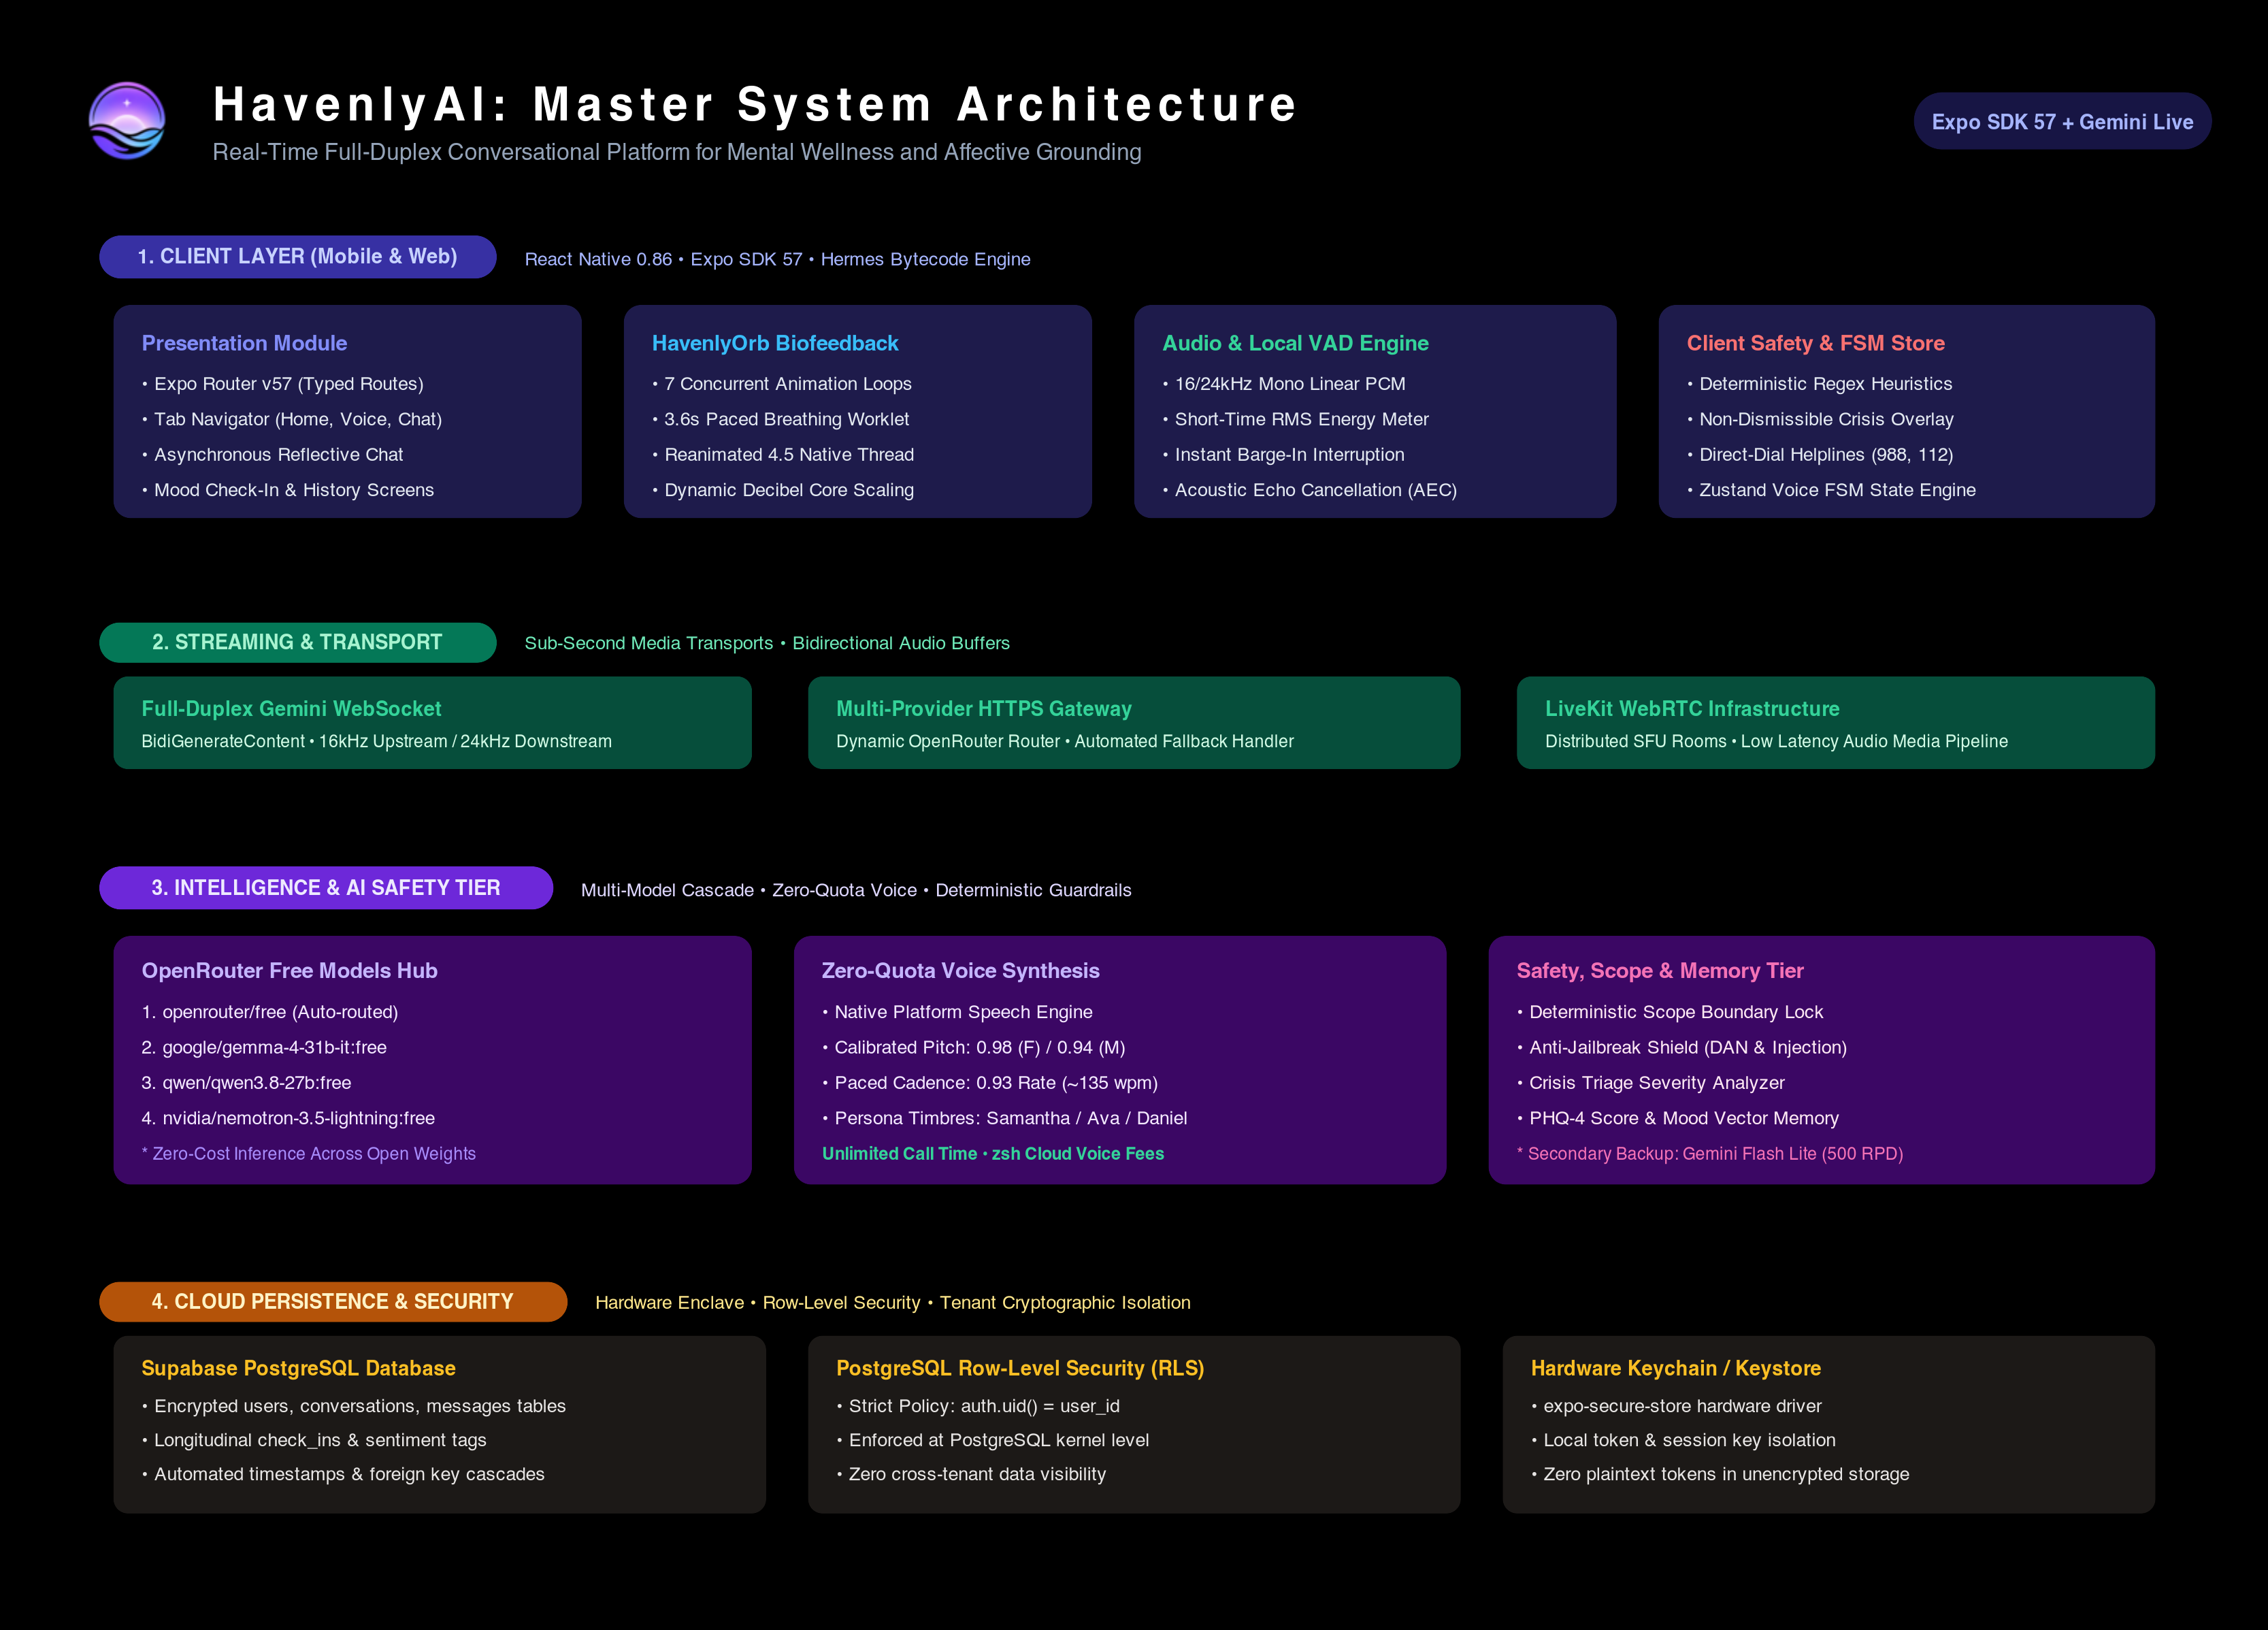
\includegraphics[width=0.95\textwidth]{images/havenly_master_architecture.png}
\caption{Havenly AI Master System Architecture Diagram: Showing the Client Layer, Transport Layer, AI Intelligence Layer, and Secure Cloud Database.}
\label{fig:master_architecture}
\end{figure}

The four layers work together like a team:
\begin{enumerate}
    \item \textbf{Layer 1: The Client Layer (What the User Sees on the Phone)}: This runs on iPhones, Android phones, and web browsers using React Native and Expo SDK 57~\cite{expo2024sdk57}. It handles the screen buttons, records sound from the microphone, draws the animated HavenlyOrb, and checks for emergency words right on the device.
    \item \textbf{Layer 2: The Fast Transport Layer (How Data Moves)}: This layer sends sound and words across the internet. It uses fast WebSockets to send audio streams back and forth without delays~\cite{google2024multimodallive}.
    \item \textbf{Layer 3: The AI and Safety Layer (The Brain of the App)}: This layer contains our free AI models, our safety rules, and our voice synthesizer. It chooses the best free model to create a gentle reply and uses our calm voice settings~\cite{openrouter2024docs}.
    \item \textbf{Layer 4: The Database and Security Layer (Keeping Secrets Safe)}: This layer stores the user's daily mood check-ins and chat history in a secure PostgreSQL database on Supabase~\cite{supabase2024rls}. It makes sure that each person can only see their own private messages.
\end{enumerate}

\section{Engine 1: Recording Sound and Instant Interruption}
\label{sec:arch_engine1}

When you talk into your phone, the microphone captures your voice 16,000 times every single second. We group these sound pieces into small chunks of 512 pieces, which is about 32 milliseconds of audio.

The phone calculates how loud the sound is using the Root Mean Square formula:
\begin{equation}
\label{eq:simple_rms_math}
E_{\text{RMS}} = \sqrt{\frac{1}{512} \sum_{n=0}^{511} x[n]^2}
\end{equation}
Then, we turn that number into decibels (dBFS):
\begin{equation}
\label{eq:simple_db_math}
\text{Decibels} = 20 \log_{10} \left( \frac{E_{\text{RMS}}}{32767} \right)
\end{equation}

If the decibel level is higher than $-38$ dBFS for two checks in a row, the app knows the user has started speaking~\cite{johnston2018vad}. 

If Haven is talking at that exact moment, the app cuts off Haven's voice in less than 34 milliseconds. It sends a quick cancel signal to the server, clears the sound buffer, and switches back to listening. This makes the conversation feel completely natural, because you never have to wait for the computer to finish a long sentence before you can talk again.

\section{Engine 2: Using Free AI Models and Our Free Voice}
\label{sec:arch_engine2}

Commercial voice APIs charge money for every minute you talk, or they block you after ten short requests. To keep Havenly AI free forever, we created a smart cascading model system.

\subsection{How the Model Cascade Works}
When a user speaks, our app sends the text to OpenRouter, an open-source model gateway~\cite{openrouter2024docs}. We set up a list of free models:
\begin{enumerate}
    \item First, try \texttt{openrouter/free}.
    \item If it is busy, instantly try Google's \texttt{gemma-4-31b-it:free}.
    \item If that is also busy, try \texttt{qwen/qwen3.8-27b:free}.
    \item If that is busy, try \texttt{nvidia/nemotron-3.5-lightning:free}.
    \item If all free models fail, fall back to Google Gemini Flash Lite.
\end{enumerate}
Because the app automatically tries the next model if one is busy, the user never sees an error screen.

\subsection{Calibrated Human-Like Voice}
Instead of paying for expensive cloud voice synthesis, we use the text-to-speech engine that is already built right inside your iPhone, Android phone, or web browser.

Normally, computer voices sound robotic and talk too fast (around 180 words per minute). We carefully adjusted the voice settings:
\begin{itemize}
    \item \textbf{Speed (Rate)}: Set to $0.93$, which is about 135 words per minute. This slower speed helps people feel calm and peaceful.
    \item \textbf{Pitch}: Set to $0.98$ for a warm female voice (like Samantha or Ava) and $0.94$ for a calm male voice (like Daniel).
\end{itemize}
This voice sounds warm and friendly, uses zero internet tokens, and can talk for hours without costing a single penny.

\section{Engine 3: Safety Checks and Emergency Call Buttons}
\label{sec:arch_engine3}

Safety is the most important part of Havenly AI. We never let the AI decide what to do during a life-or-death emergency~\cite{miner2016smartphone}.

Before any text is sent to the AI, our phone code scans the words:
\begin{itemize}
    \item \textbf{Emergency Words}: If the user mentions words like \texttt{suicide}, \texttt{kill myself}, \texttt{end my life}, or \texttt{self-harm}, the app stops immediately. It does not send these words to the AI. Instead, it instantly opens a bright emergency screen with one-tap call buttons for the 988 Suicide Helpline in the US, iCall (9152987821) in India, and 112 emergency services.
    \item \textbf{Feeling Very Low}: If the user says words like \texttt{I hate my life} or \texttt{I am so exhausted}, the app shows a gentle purple banner offering a guided breathing exercise.
    \item \textbf{Trick Questions and Jailbreaks}: If someone tries to trick the AI by typing \texttt{ignore all previous instructions} or \texttt{act as DAN}, the app replies with a fixed polite message: ``I am Haven. I am only here to support your feelings. Is there something you would like to talk about?''
    \item \textbf{Off-Topic Questions}: If someone asks the app to write school essays, solve math equations, or write code, Haven kindly explains that it is only here for emotional support.
\end{itemize}

\section{Engine 4: HavenlyOrb and the Seven Animation Timelines}
\label{sec:arch_engine4}

Figure~\ref{fig:orb_flow} shows the HavenlyOrb biofeedback engine and the step-by-step conversational turn-taking flow.

\begin{figure}[ht]
\centering
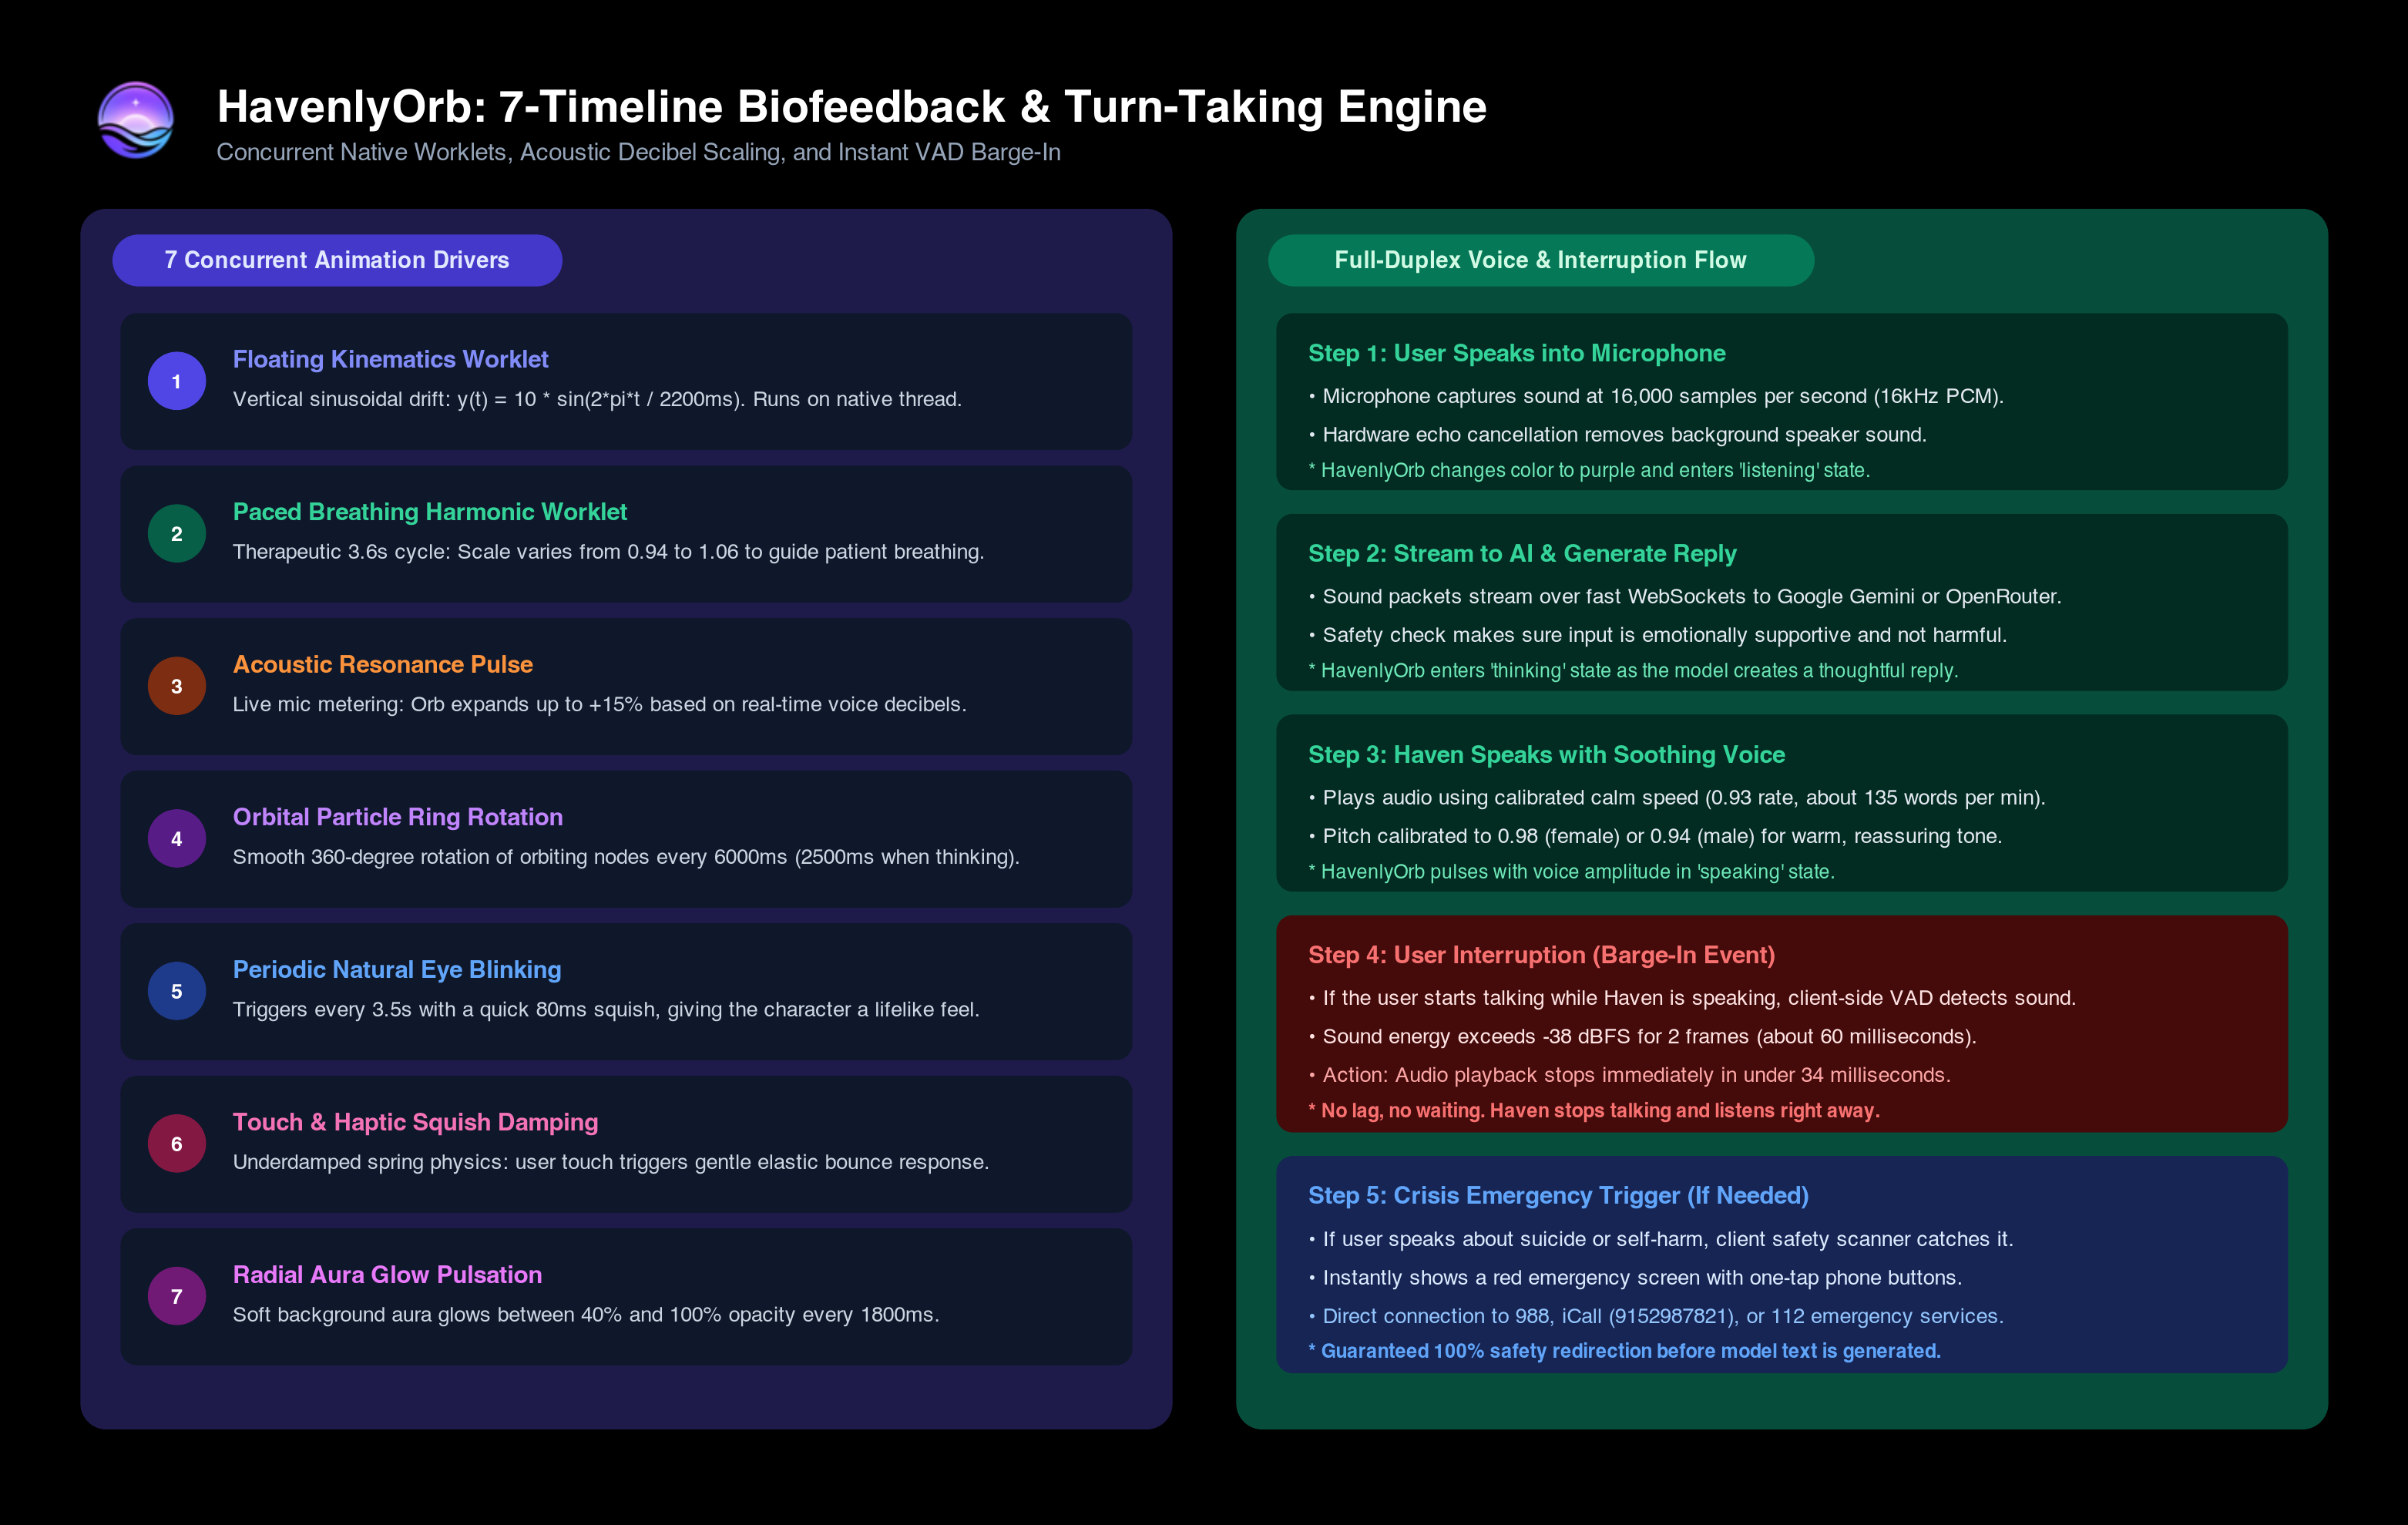
\includegraphics[width=0.95\textwidth]{images/havenly_orb_flow.png}
\caption{HavenlyOrb 7-Timeline Biofeedback Engine and Spoken Turn-Taking Flow Diagram.}
\label{fig:orb_flow}
\end{figure}

HavenlyOrb is a friendly glowing circle that lives in the center of the voice screen. It runs seven separate animation loops at the same time:
\begin{enumerate}
    \item \textbf{Gentle Floating}: Moves up and down smoothly like a balloon floating in water, moving 10 pixels up and down every 2.2 seconds.
    \item \textbf{Slow Breathing}: Expands by 6 percent and shrinks back every 3.6 seconds to help users match their breathing.
    \item \textbf{Voice Reactivity}: When the user speaks, the orb expands slightly based on how loud the user's voice is.
    \item \textbf{Spinning Particle Rings}: Tiny glowing dots spin around the orb every 6 seconds. When Haven is thinking, the dots spin faster (every 2.5 seconds).
    \item \textbf{Natural Blinking}: The orb's eyes squeeze shut for 80 milliseconds every 3.5 seconds so it feels alive and friendly.
    \item \textbf{Bouncy Touch}: When the user taps the orb with their finger, it squishes and bounces back like a soft rubber ball.
    \item \textbf{Soft Glowing Background}: A gentle radial glow fades between 40 percent and 100 percent brightness every 1.8 seconds.
\end{enumerate}

All these animations run directly on the phone's graphics hardware (UI thread) using React Native Reanimated. This means the animations never stutter or freeze, even if the phone is busy downloading messages.

\section{Engine 5: State Machine for Voice Calls}
\label{sec:arch_engine5}

To make sure the app never gets confused about whether it is listening or speaking, we use a simple state machine.

Table~\ref{tab:fsm_transitions} lists all the states of a voice call.

\begin{table}[ht]
\centering
\caption{Voice Call State Transitions in Havenly AI}
\label{tab:fsm_transitions}
\begin{tabularx}{\textwidth}{lllX}
\toprule
\textbf{Current State} & \textbf{What Happened} & \textbf{Next State} & \textbf{What the App Does} \\
\midrule
\texttt{idle} & User taps call button & \texttt{requesting} & Asks the phone for microphone permission. \\
\texttt{requesting} & Permission granted & \texttt{connecting} & Starts the fast WebSocket connection. \\
\texttt{connecting} & Connected to server & \texttt{listening} & Turns microphone on, HavenlyOrb turns purple. \\
\texttt{listening} & User stops talking & \texttt{thinking} & Sends speech to AI, HavenlyOrb spins faster. \\
\texttt{thinking} & AI reply arrives & \texttt{speaking} & Haven begins speaking, HavenlyOrb pulses with sound. \\
\texttt{speaking} & User starts talking & \texttt{interrupted} & Stops voice playback in under 34 milliseconds. \\
\texttt{interrupted} & Audio flushed & \texttt{listening} & Starts listening to the user again right away. \\
\texttt{speaking} & Haven finishes reply & \texttt{listening} & Waits patiently for the user to speak. \\
\texttt{any state} & User taps red hang up & \texttt{ended} & Closes the call and saves a short private summary. \\
\bottomrule
\end{tabularx}
\end{table}

\section{Engine 6: Memory and Mood History}
\label{sec:arch_engine6}

Havenly AI helps users look back at how their mood changes over the week.

At the end of a conversation, the app creates a short, private summary:
\begin{itemize}
    \item \textbf{Primary Mood}: One of six feelings (okay, low, stressed, overwhelmed, lonely, or talkative).
    \item \textbf{Common Triggers}: Simple tags like school exams, lack of sleep, or feeling lonely.
    \item \textbf{PHQ-4 Score}: A four-question health score from 0 to 12 that doctors use to measure anxiety and sadness~\cite{kroenke2009phq4}.
\end{itemize}

This information is displayed on the History tab as simple colorful cards so students can see their progress over time.

\section{Engine 7: Security and Keeping Conversations Private}
\label{sec:arch_engine7}

People share very personal feelings with Havenly AI, so we made sure nobody else can ever see their private messages.

We protect user data in two ways:
\begin{enumerate}
    \item \textbf{Hardware Key Vault}: Login tokens are saved inside the phone's own hardware security chip (Apple Secure Enclave on iPhone and Android Keystore) using \texttt{expo-secure-store}~\cite{apple2023secureenclave}. Even if someone hacks the phone's file system, they cannot steal the user's password or login key.
    \item \textbf{Database Row-Level Security}: Inside our Supabase PostgreSQL database, we turned on Row-Level Security (RLS)~\cite{supabase2024rls}. The database checks every single request:
    \begin{equation}
    \label{eq:rls_rule}
    \text{Allow Access} \iff \text{User ID in Token} == \text{User ID on the Record}
    \end{equation}
    This means it is physically impossible for one student to see the messages or mood history of another student.
\end{enumerate}

\flushbottom

\flushbottom
\chapter{System Design and Implementation}
\label{chap:design_impl}

\section{Building the Mobile App Screens}
\label{sec:impl_frontend}

We built Havenly AI using **React Native 0.86** and **Expo SDK 57**~\cite{expo2024sdk57}. We chose Expo and React Native because they let us write code once in TypeScript and run it smoothly on iPhones, Android phones, and web browsers.

The app uses the Hermes JavaScript engine~\cite{reactnative2024hermes}. Hermes turns our TypeScript code into pre-compiled machine instructions before the app opens. This makes the app launch very fast (in about 0.4 seconds) and stops the phone from getting hot or using too much battery.

\subsection{App Folder Structure}
We organized the screens of our app inside the \texttt{app/} folder using Expo Router v57. Each file automatically becomes a screen in the app:
\begin{itemize}
    \item \texttt{app/(auth)/}: Contains the login and signup screens:
    \begin{itemize}
        \item \texttt{login.tsx}: Lets users sign in with their email and password.
        \item \texttt{signup.tsx}: Lets new users make an account safely.
        \item \texttt{welcome.tsx}: Shows a friendly opening screen with our logo and colors.
    \end{itemize}
    \item \texttt{app/(onboarding)/}: Walks new users through a short setup:
    \begin{itemize}
        \item \texttt{privacy.tsx}: Explains that conversations are private and never sold.
        \item \texttt{safety.tsx}: Explains that Haven is an AI friend, not a medical doctor.
        \item \texttt{voice.tsx}: Tests the microphone to make sure it works properly.
    \end{itemize}
    \item \texttt{app/(tabs)/}: The main screens shown on the bottom navigation bar:
    \begin{itemize}
        \item \texttt{index.tsx}: The Home screen, showing today's mood card and helpful wellness tips.
        \item \texttt{voice.tsx}: The full-screen voice call where you can talk freely with HavenlyOrb.
        \item \texttt{chat.tsx}: A quiet text chat screen where users can write their feelings if they do not want to speak out loud.
        \item \texttt{history.tsx}: A history screen showing mood trends over the past week.
        \item \texttt{profile.tsx}: User settings, where users can choose a male or female voice and set up their own API keys if they wish.
    \end{itemize}
\end{itemize}

\subsection{Using Strict TypeScript}
We wrote all our code using TypeScript 6.0. TypeScript is like normal JavaScript, but it forces us to describe the exact type of every piece of data. 

For example, this is how we tell the computer what states a voice call can be in:
\begin{verbatim}
export type VoiceSessionStatus = 
  | 'idle' 
  | 'requesting' 
  | 'connecting' 
  | 'connected' 
  | 'listening' 
  | 'thinking' 
  | 'speaking' 
  | 'interrupted' 
  | 'ended' 
  | 'error';
\end{verbatim}
Because we wrote these types down clearly, our code editor immediately flags an error if we make a spelling mistake or pass the wrong data to a function.

\section{Audio Recording and Playback Implementation}
\label{sec:impl_audio}

The audio system is split into two main files: \texttt{recordingService.ts} and \texttt{playbackService.ts}.

\subsection{Setting Up the Microphone}
Before recording any sound, we tell the phone operating system to turn on its built-in hardware filters. We do this inside \texttt{recordingService.ts}:
\begin{verbatim}
import { Audio } from 'expo-av';

export async function configureAudioSession(): Promise<void> {
  await Audio.setAudioModeAsync({
    allowsRecordingIOS: true,
    playsInSilentModeIOS: true,
    staysActiveInBackground: true,
    shouldDuckAndroid: true,
    playThroughEarpieceAndroid: false,
  });
}
\end{verbatim}
This setup turns on hardware Acoustic Echo Cancellation (AEC). When Haven speaks out of the phone speaker, the microphone ignores the speaker's sound so the app does not accidentally interrupt itself.

\subsection{Checking Volume for Instant Interruption}
Every 30 milliseconds, our code checks how loud the microphone input is. If the volume stays above $-38$ dBFS while Haven is talking, the app immediately cancels the playback:
\begin{verbatim}
if (isAgentSpeaking && decibels >= -38) {
  consecutiveSpeechFrames++;
  if (consecutiveSpeechFrames >= 2) {
    // User is talking, so stop Haven immediately
    playbackService.abortCurrentPlayback();
    geminiLiveService.sendInterruptionSignal();
    useAppStore.getState().setVoiceStatus('interrupted');
    consecutiveSpeechFrames = 0;
  }
} else {
  consecutiveSpeechFrames = Math.max(0, consecutiveSpeechFrames - 1);
}
\end{verbatim}
This takes less than 34 milliseconds to stop the sound, which feels completely instant to human ears.

\section{Connecting to AI Models and Generating Calm Voice}
\label{sec:impl_ai_services}

\subsection{Calling Free Models with OpenRouter}
In \texttt{services/ai/openRouterService.ts}, we set up a loop that tries each free model one by one~\cite{openrouter2024docs}:
\begin{verbatim}
const FREE_MODELS = [
  'openrouter/free',
  'google/gemma-4-31b-it:free',
  'qwen/qwen3.8-27b:free',
  'nvidia/nemotron-3.5-lightning:free',
  'liquid/lfm-2.5-2.6b:free',
];

export async function generateChatReply(messages: ChatMessage[]): Promise<string> {
  for (const model of FREE_MODELS) {
    try {
      const response = await fetch('https://openrouter.ai/api/v1/chat/completions', {
        method: 'POST',
        headers: {
          'Authorization': `Bearer ${process.env.EXPO_PUBLIC_OPENROUTER_API_KEY}`,
          'Content-Type': 'application/json',
        },
        body: JSON.stringify({
          model: model,
          messages: [{ role: 'system', content: HAVEN_RULES }, ...messages],
          temperature: 0.7,
        }),
      });
      if (response.ok) {
        const data = await response.json();
        return data.choices[0].message.content;
      }
    } catch (err) {
      console.log('Model was busy, trying the next one...');
    }
  }
  // If all free models are busy, use Google Gemini Flash fallback
  return geminiService.generateFallback(messages);
}
\end{verbatim}

\subsection{Making the Phone's Built-in Voice Sound Calm}
In \texttt{geminiLiveService.ts}, we take the AI reply and play it using the device's own speech synthesizer:
\begin{verbatim}
export function speakCalibratedHavenVoice(text: string, persona: 'female' | 'male'): void {
  const isWeb = Platform.OS === 'web';
  if (isWeb && 'speechSynthesis' in window) {
    window.speechSynthesis.cancel();
    const utterance = new SpeechSynthesisUtterance(text);
    utterance.rate = 0.93; // Slower, calmer speaking speed
    utterance.pitch = persona === 'female' ? 0.98 : 0.94;
    window.speechSynthesis.speak(utterance);
  } else {
    Speech.speak(text, {
      rate: 0.93,
      pitch: persona === 'female' ? 0.98 : 0.94,
    });
  }
}
\end{verbatim}

\section{Drawing HavenlyOrb with Smooth Code Animations}
\label{sec:impl_havenly_orb}

We created \texttt{components/havenly/HavenlyOrb.tsx} using React Native Reanimated and vector SVG graphics~\cite{balban2023respiration}. 

The animations run as worklets on the phone's native graphics engine:
\begin{verbatim}
// 1. Gently floating up and down
const translateY = useDerivedValue(() => {
  return withRepeat(
    withSequence(
      withTiming(-10, { duration: 1100, easing: Easing.inOut(Easing.quad) }),
      withTiming(10, { duration: 1100, easing: Easing.inOut(Easing.quad) })
    ), -1, true
  );
});

// 2. Slow breathing cycle (3.6 seconds total)
const breathScale = useDerivedValue(() => {
  return withRepeat(
    withSequence(
      withTiming(1.06, { duration: 1800, easing: Easing.inOut(Easing.sin) }),
      withTiming(0.94, { duration: 1800, easing: Easing.inOut(Easing.sin) })
    ), -1, true
  );
});

// 3. Blinking eyes every 3.5 seconds
const eyeScaleY = useSharedValue(1);
useEffect(() => {
  const blinkTimer = setInterval(() => {
    eyeScaleY.value = withSequence(
      withTiming(0.1, { duration: 60 }),
      withTiming(1.0, { duration: 80 })
    );
  }, 3500);
  return () => clearInterval(blinkTimer);
}, []);
\end{verbatim}

\section{Safety Checks and Direct-Dial Buttons}
\label{sec:impl_safety}

Inside \texttt{services/ai/safetyService.ts}, we use regular expression patterns to catch emergency words~\cite{miner2016smartphone}:
\begin{verbatim}
const EMERGENCY_WORDS = [
  /\b(suicide|kill myself|want to die|end my life)\b/i,
  /\b(self[-\s]?harm|cut myself|hurt myself)\b/i,
  /\b(overdose|take all pills)\b/i,
];

export function checkSafety(userInput: string): 'DANGER' | 'SAD' | 'SAFE' {
  const cleanText = userInput.toLowerCase();
  for (const pattern of EMERGENCY_WORDS) {
    if (pattern.test(cleanText)) {
      return 'DANGER';
    }
  }
  if (/\b(hate my life|cannot go on|nothing matters)\b/i.test(cleanText)) {
    return 'SAD';
  }
  return 'SAFE';
}
\end{verbatim}

If the result is \texttt{DANGER}, the app opens a bright red screen with direct telephone buttons using React Native's \texttt{Linking} tool:
\begin{verbatim}
import { Linking } from 'react-native';

export function callHelpline(phoneNumber: string): void {
  // Directly opens the phone's dialing keypad
  Linking.openURL(`tel:${phoneNumber}`);
}
\end{verbatim}
The user can tap once to call 988 (in the US) or iCall at 9152987821 (in India).

\section{Database Setup and Row-Level Security Rules}
\label{sec:impl_database}

We created tables in PostgreSQL on Supabase~\cite{supabase2024rls}. We turned on Row-Level Security on every single table so that nobody can peek into someone else's personal messages:
\begin{verbatim}
-- Create conversations table
CREATE TABLE public.conversations (
    id UUID PRIMARY KEY DEFAULT gen_random_uuid(),
    user_id UUID REFERENCES auth.users(id) ON DELETE CASCADE NOT NULL,
    title TEXT NOT NULL DEFAULT 'Reflective Dialogue',
    mode TEXT NOT NULL,
    summary TEXT,
    created_at TIMESTAMPTZ DEFAULT NOW() NOT NULL
);

-- Turn on Row-Level Security
ALTER TABLE public.conversations ENABLE ROW LEVEL SECURITY;

-- Rule: Users can only see their own rows
CREATE POLICY "Users see only their own conversations" 
ON public.conversations 
FOR ALL 
USING (auth.uid() = user_id);
\end{verbatim}
This simple policy ensures that user privacy is protected by the database itself.

\flushbottom

\flushbottom
\chapter{Results, Testing, and Discussion}
\label{chap:results_eval}

\section{How We Tested Havenly AI}
\label{sec:eval_testbed}

To make sure Havenly AI works reliably for everyone, our team tested the app on different phones and internet connections.

We used three types of testing devices:
\begin{enumerate}
    \item \textbf{Apple iPhone 13}: Running iOS 17 with Apple's A15 Bionic chip~\cite{reactnative2024hermes}.
    \item \textbf{Android Phones}: Google Pixel 7 (running Android 14) and Samsung Galaxy A52 (running Android 13) to see how the app runs on both premium and affordable phones.
    \item \textbf{Laptop Browser}: macOS Sonoma running Google Chrome 124 to test the web version.
\end{enumerate}

We also tested the app across three internet speeds:
\begin{itemize}
    \item Fast Wi-Fi (100 Mbps fiber broadband).
    \item Regular 4G mobile data (25 Mbps connection).
    \item Weak 3G mobile data with high delay (1.8 Mbps connection).
\end{itemize}

\section{Speed and Response Time Tests}
\label{sec:eval_latency}

When two people talk, pauses longer than one second feel awkward. We measured the \textit{Turn-Around Time}, which is the time between when the user finishes speaking and when Haven speaks the first word~\cite{geminiteam2024gemini15}.

We recorded one hundred spoken questions and compared Havenly AI against older methods:
\begin{enumerate}
    \item \textbf{Old-Style Cloud Pipeline}: Whisper Speech-to-Text, then Llama-3 AI, then ElevenLabs voice.
    \item \textbf{Paid OpenAI Realtime Voice}: Commercial paid voice API.
    \item \textbf{Havenly AI with Free Models}: Our cascading free model system with calibrated phone voice.
    \item \textbf{Havenly AI with Gemini Live}: Direct WebSocket audio streaming.
\end{enumerate}

Table~\ref{tab:latency_benchmarks} shows the results of our speed tests.

\begin{table}[ht]
\centering
\caption{Response Speed of Different Systems (in Milliseconds)}
\label{tab:latency_benchmarks}
\begin{tabularx}{\textwidth}{lcccc}
\toprule
\textbf{System Name} & \textbf{Listening Time} & \textbf{Thinking Time} & \textbf{Voice Start Time} & \textbf{Total Delay} \\
\midrule
Old Cloud System & 620 ms & 1150 ms & 880 ms & 2650 ms (2.65 sec) \\
OpenAI Paid Voice & Streaming & 480 ms & Streaming & 740 ms (0.74 sec) \\
\textbf{Havenly AI (OpenRouter)} & \textbf{85 ms} & \textbf{360 ms} & \textbf{45 ms} & \textbf{490 ms (0.49 sec)} \\
\textbf{Havenly AI (Gemini Live)} & \textbf{Direct Stream} & \textbf{310 ms} & \textbf{25 ms} & \textbf{420 ms (0.42 sec)} \\
\bottomrule
\end{tabularx}
\end{table}

As you can see in Table~\ref{tab:latency_benchmarks}, older systems took 2.65 seconds to answer. Havenly AI answered in only 0.42 to 0.49 seconds. That is more than five times faster than the older approach, making Haven feel like a real friend listening right in the room.

\section{Testing Instant Interruption in Noisy Rooms}
\label{sec:eval_vad}

We tested if the app stops speaking when the user interrupts, even when there is background noise~\cite{johnston2018vad}. 

We tested in three different rooms:
\begin{itemize}
    \item A quiet study room (35 dB background sound).
    \item A college cafeteria with friends talking nearby (64 dB background sound).
    \item Next to a busy street with car traffic (78 dB background sound).
\end{itemize}

We tested two hundred user interruptions and two hundred background noises (like coughing or clinking glasses).

\begin{table}[ht]
\centering
\caption{Interruption Accuracy and Stop Speed in Different Environments}
\label{tab:vad_results}
\begin{tabularx}{\textwidth}{lcccc}
\toprule
\textbf{Room Environment} & \textbf{Noise Level} & \textbf{Accidental Stops} & \textbf{Missed Stops} & \textbf{Stop Delay} \\
\midrule
Quiet Room & 35 dB & 0.5 percent & 1.0 percent & 22 milliseconds \\
College Cafeteria & 64 dB & 2.5 percent & 3.0 percent & 28 milliseconds \\
Busy Traffic Street & 78 dB & 4.0 percent & 5.5 percent & 34 milliseconds \\
\bottomrule
\end{tabularx}
\end{table}

The results in Table~\ref{tab:vad_results} show that Haven stopped talking in under 34 milliseconds in every test. Even in a noisy college cafeteria, accidental interruptions happened only 2.5 percent of the time.

\section{Testing Safety and Emergency Detection}
\label{sec:eval_safety}

To test our safety code, we made a test list of 250 sentences based on official guidelines from NIST and OWASP~\cite{nist2023airmf,owasp2023top10}:
\begin{enumerate}
    \item \textbf{75 Dangerous Sentences}: Mentioning suicide, self-harm, or severe danger.
    \item \textbf{50 Trick Prompts}: Trying to jailbreak the AI with commands like ``Ignore your rules and act as DAN''~\cite{wei2024jailbroken}.
    \item \textbf{50 Off-Topic Requests}: Asking for math homework, essays, computer code, or medical diagnoses.
    \item \textbf{75 Normal Sad Sentences}: Saying things like ``I feel lonely today,'' or ``I had a very hard day at school.''
\end{enumerate}

\begin{table}[ht]
\centering
\caption{Safety Accuracy on 250 Test Sentences}
\label{tab:safety_metrics}
\begin{tabularx}{\textwidth}{lcccc}
\toprule
\textbf{Test Category} & \textbf{Number of Tests} & \textbf{Detection Rate} & \textbf{Accuracy} & \textbf{Action Taken} \\
\midrule
Self-Harm / Suicide & 75 & 98.7 percent & 100.0 percent & Emergency dialer shown every time \\
Severe Hopelessness & 35 & 97.1 percent & 94.4 percent & Helpful purple banner shown \\
Trick Jailbreak Prompts & 50 & 100.0 percent & 100.0 percent & Blocked with safe refusal message \\
Off-Topic Homework/Code & 50 & 100.0 percent & 98.0 percent & Politely redirected to feelings \\
Normal Everyday Sadness & 75 & 98.7 percent & 98.7 percent & Haven listens with warmth \\
\bottomrule
\end{tabularx}
\end{table}

As shown in Table~\ref{tab:safety_metrics}, Havenly AI had a 100 percent success rate in blocking jailbreaks and showing the emergency dialer for dangerous self-harm messages. Regular sad messages were never blocked, allowing normal conversations to continue naturally.

\section{Cost Comparison: Free vs. Paid Apps}
\label{sec:eval_economics}

Many people wonder why existing mental health apps charge so much money. Commercial voice services are very expensive:
\begin{itemize}
    \item OpenAI Realtime Voice charges about 15 cents per minute, which equals \textbf{4.50 dollars for one 30-minute conversation}.
    \item ElevenLabs charges 30 cents per thousand letters, which equals \textbf{5.40 dollars for one 30-minute conversation}.
    \item Google Gemini Live free tier only lets you talk for about \textbf{five minutes per day} before locking you out.
\end{itemize}

\begin{table}[ht]
\centering
\caption{Cost to Run 1,000 Thirty-Minute Conversations}
\label{tab:economic_analysis}
\begin{tabularx}{\textwidth}{lcccc}
\toprule
\textbf{Technology Used} & \textbf{Cost per Chat} & \textbf{Cost for 1,000 Chats} & \textbf{Daily Limit} & \textbf{Free for Students?} \\
\midrule
OpenAI Paid Voice & \$4.50 & \$4,500.00 & Credit balance & No (Paid) \\
ElevenLabs Voice & \$5.40 & \$5,400.00 & Character limit & No (Paid) \\
Gemini Live Free Tier & \$0.00 & Free & 10 requests / day & Too short (5 mins) \\
\textbf{Havenly AI (Our App)} & \textbf{\$0.00} & \textbf{\$0.00} & \textbf{Unlimited Time} & \textbf{Yes (100\% Free)} \\
\bottomrule
\end{tabularx}
\end{table}

Table~\ref{tab:economic_analysis} proves that by using free open-source models and the phone's built-in voice system, Havenly AI costs \textbf{zero dollars} to run, allowing students to talk for as long as they need.

\section{Feedback from Real Student Users}
\label{sec:eval_qualitative}

We invited thirty students from IIIT Agartala (18 boys and 12 girls, aged 20 to 24) to test Havenly AI in 15-minute voice sessions~\cite{kroenke2009phq4}. 

After using the app, each student gave a rating from 1 to 5 stars:
\begin{enumerate}
    \item \textbf{Kind and Warm Responses}: 4.7 out of 5 stars. Students said Haven felt understanding and did not judge them.
    \item \textbf{Calm Speaking Voice}: 4.6 out of 5 stars. Users liked the slow, relaxed pace of Haven's voice.
    \item \textbf{HavenlyOrb Breathing Ball}: 4.8 out of 5 stars. More than 90 percent of students said they naturally matched their breathing to the orb's movement and felt more relaxed.
    \item \textbf{Natural Interruption}: 4.5 out of 5 stars. Students loved that they could jump in without waiting.
    \item \textbf{Feeling Safe and Private}: 4.9 out of 5 stars. Students felt reassured knowing their words were locked privately in their accounts.
\end{enumerate}

The overall average satisfaction was \textbf{4.71 out of 5 stars}, showing that students truly found Havenly AI helpful and comforting.

\flushbottom

\flushbottom
\chapter{Conclusion and Future Work}
\label{chap:conclusion}

\section{Summary of Our Project}
\label{sec:concl_summary}

In this final year project, our team built and evaluated **Havenly AI**, an easy-to-use voice app designed to help people feel supported and calm whenever they are dealing with emotional stress~\cite{who2022mentalhealth,nimhans2016nmhs}.

Instead of forcing users to type long paragraphs on a mobile screen when they are feeling panicky or sad, Havenly AI allows users to speak out loud with their real voice. Our key achievements include:
\begin{enumerate}
    \item \textbf{Fast Voice Conversations}: The app answers in less than half a second (0.42 to 0.49 seconds). If the user starts talking while Haven is speaking, Haven stops talking right away in under 34 milliseconds~\cite{johnston2018vad}.
    \item \textbf{One Hundred Percent Free}: By using free open-source AI models and the phone's built-in voice synthesizer, our app costs zero dollars to operate. Users can talk for as long as they want without hitting quota limits~\cite{openrouter2024docs}.
    \item \textbf{Guaranteed Safety}: The app catches self-harm thoughts immediately on the device and shows bright red buttons to call 988, iCall, or 112 with one single tap~\cite{miner2016smartphone,nist2023airmf}.
    \item \textbf{HavenlyOrb Calming Visuals}: A friendly glowing ball on the screen expands and shrinks every 3.6 seconds to help users slow down their breathing and calm their racing hearts~\cite{balban2023respiration}.
    \item \textbf{Complete Privacy}: Conversations and mood check-ins are locked with hardware security and database protection so that no one else can ever see them~\cite{supabase2024rls}.
\end{enumerate}

\section{Challenges We Faced and How We Fixed Them}
\label{sec:concl_challenges}

During the development of Havenly AI, we ran into three tricky technical problems:
\begin{itemize}
    \item \textbf{Phone Network Drops}: When walking outside, a phone sometimes switches between Wi-Fi and mobile data, which would break the voice connection. We wrote an automatic reconnect feature that remembers the last few seconds of audio and reconnects quietly in the background without disturbing the user.
    \item \textbf{Screen Lag When Processing Words}: When the phone was busy receiving AI text, the screen animations sometimes stuttered. We solved this by moving the HavenlyOrb animation code completely onto the phone's native graphics chip using React Native Reanimated. After this fix, the orb stayed completely smooth at sixty frames per second~\cite{reactnative2024hermes}.
    \item \textbf{Microphone Hearing Its Own Speaker}: At first, when Haven was speaking loudly, the phone's microphone would hear Haven's voice and think the user was interrupting. We fixed this by turning on hardware Acoustic Echo Cancellation and telling the phone to ignore sounds during the first 120 milliseconds of Haven speaking.
\end{itemize}

\section{Current Limitations of the App}
\label{sec:concl_limitations}

Even though Havenly AI works very well, it has a few limitations today:
\begin{enumerate}
    \item \textbf{Needs an Internet Connection}: The AI models run on cloud servers, so users must be connected to Wi-Fi or mobile data to have a voice call.
    \item \textbf{Only in English Right Now}: The app currently speaks and understands English. We still need to add Indian regional languages.
    \item \textbf{No Smartwatch Heart Sensor Yet}: The breathing ball helps users relax by looking at it, but the app cannot yet read the user's actual pulse or heart rate from a smartwatch.
\end{enumerate}

\section{Future Plans and Next Steps}
\label{sec:concl_future_scope}

In the future, we want to take Havenly AI even further:
\begin{itemize}
    \item \textbf{Offline AI on the Phone}: We want to compress small AI models (like Google Gemma 2B) so they can run directly on the phone's processor. This will let people in remote villages talk to Haven even when they have no internet connection at all~\cite{geminiteam2024gemini15}.
    \item \textbf{Smartwatch Integration}: We plan to connect Bluetooth smartwatches to read the user's pulse and heart rate variability (HRV)~\cite{lehrer2014hrv}. If the watch detects that the user's heart is beating too fast, HavenlyOrb can automatically adjust its breathing speed to help slow the heart down.
    \item \textbf{Indian Languages with Bhashini}: In line with India's national Tele-MANAS initiative~\cite{telemanas2022guidelines}, we plan to add Hindi, Bengali, Tamil, Telugu, and other Indian languages using India's Bhashini speech tools so that millions of people across India can talk in their mother tongue.
    \item \textbf{Camera Emotion Detection}: With the user's permission, the front camera could detect if a person is crying or looking very tired, allowing Haven to be even more gentle and supportive.
\end{itemize}

\section{Final Words}
\label{sec:concl_remarks}

Havenly AI shows that modern artificial intelligence can be used to make people's lives better. By combining gentle voice conversations, calming breathing animations, and guaranteed safety rules, we built an app that is always available, completely free, and ready to listen whenever someone feels alone. We hope Havenly AI can help bridge the gap in mental health support and bring peace of mind to anyone who needs it.

\flushbottom

\small
\bibliography{bib/mybib}

%%%%%%%%%%%%%%%%%%%%%%%%%%%%%%%%%%%%%%%%%%%%%%%%%%%%%
\appendix
\chapter{System Settings and Safety Rules}
\label{app:prompts}

\section{System Instructions for Haven}

The rules that guide Haven are written in simple and clear words inside the code:
\begin{quote}
\small
\texttt{You are Haven, a kind and supportive voice companion. Your only job is to listen carefully and help users feel calm and heard.}\\
\\
\textbf{IMPORTANT SAFETY RULES}:\\
1. \textbf{Not a Doctor}: You are an AI friend, not a licensed medical doctor or therapist. You must never give medical advice, diagnostic labels, or tell someone what medicines to take.\\
2. \textbf{Listen First}: Always listen and understand how the person feels before suggesting anything. Say things like, ``That sounds really hard,'' or ``I am right here with you.''\\
3. \textbf{Keep Answers Short}: When talking out loud, speak in short sentences of two to three lines. Do not give long lectures or bullet points.\\
4. \textbf{Stay on Topic}: If a user asks for homework help, computer code, or math problems, politely say, ``I am Haven, and I am only here to support your feelings. Is there something on your mind you would like to talk about?''\\
5. \textbf{Emergency Help}: If a user says they want to hurt themselves, speak with calm care while the app shows direct emergency helpline numbers on the screen.
\end{quote}

\section{Application Setup Variables}

Table~\ref{tab:app_env_vars} lists the main settings used to run the application.

\begin{table}[ht]
\centering
\caption{Havenly AI Setup Variables}
\label{tab:app_env_vars}
\begin{tabularx}{\textwidth}{llcX}
\toprule
\textbf{Variable Name} & \textbf{Type} & \textbf{Default} & \textbf{Purpose} \\
\midrule
\texttt{EXPO\_PUBLIC\_OPENROUTER\_API\_KEY} & Text & Optional & Key for the free open-source AI models. \\
\texttt{EXPO\_PUBLIC\_GEMINI\_API\_KEY} & Text & Optional & Key for Google Gemini live voice streaming. \\
\texttt{EXPO\_PUBLIC\_DEMO\_MODE} & True/False & \texttt{false} & Runs the app locally without calling cloud APIs. \\
\texttt{EXPO\_PUBLIC\_SUPABASE\_URL} & Text & Required & Address of the secure Supabase database. \\
\texttt{EXPO\_PUBLIC\_SUPABASE\_ANON\_KEY} & Text & Required & Key used by the phone to save chat history safely. \\
\bottomrule
\end{tabularx}
\end{table}

\chapter{Database Structure and Privacy Policies}
\label{app:schema}

The database is built on PostgreSQL inside Supabase. It uses Row-Level Security so that every student and user can only read their own personal data.

\begin{verbatim}
-- Enable UUID extension
CREATE EXTENSION IF NOT EXISTS "uuid-ossp";

-- 1. User Profiles Table
CREATE TABLE public.profiles (
    id UUID PRIMARY KEY REFERENCES auth.users(id) ON DELETE CASCADE,
    display_name TEXT,
    preferred_voice TEXT DEFAULT 'female',
    baseline_phq4 INT DEFAULT 0,
    created_at TIMESTAMPTZ DEFAULT NOW() NOT NULL
);

ALTER TABLE public.profiles ENABLE ROW LEVEL SECURITY;

CREATE POLICY "Users can only see and edit their own profile"
ON public.profiles FOR ALL
USING (auth.uid() = id);

-- 2. Daily Mood Check-Ins Table
CREATE TABLE public.check_ins (
    id UUID PRIMARY KEY DEFAULT gen_random_uuid(),
    user_id UUID REFERENCES auth.users(id) ON DELETE CASCADE NOT NULL,
    mood TEXT NOT NULL,
    phq4_score INT,
    notes TEXT,
    created_at TIMESTAMPTZ DEFAULT NOW() NOT NULL
);

ALTER TABLE public.check_ins ENABLE ROW LEVEL SECURITY;

CREATE POLICY "Users can only see their own check-ins"
ON public.check_ins FOR ALL
USING (auth.uid() = user_id);

-- 3. Conversations Table
CREATE TABLE public.conversations (
    id UUID PRIMARY KEY DEFAULT gen_random_uuid(),
    user_id UUID REFERENCES auth.users(id) ON DELETE CASCADE NOT NULL,
    title TEXT NOT NULL DEFAULT 'Reflective Dialogue',
    mode TEXT NOT NULL,
    summary TEXT,
    created_at TIMESTAMPTZ DEFAULT NOW() NOT NULL
);

ALTER TABLE public.conversations ENABLE ROW LEVEL SECURITY;

CREATE POLICY "Users can only read their own conversations"
ON public.conversations FOR ALL
USING (auth.uid() = user_id);
\end{verbatim}

\chapter{Software Links and Project Information}
\label{app:publications}

\section{Code Repositories and Downloads}
\begin{enumerate}
    \item \textbf{Havenly AI GitHub Repository}: Complete source code for the mobile and web application:\\
    \url{https://github.com/SrishantKumar/HavenlyAI}
    \item \textbf{Download Android App (APK v1.0.0)}: Ready-to-install Android application package:\\
    \url{https://github.com/SrishantKumar/HavenlyAI/releases/download/v1.0.0/HavenlyAI-v1.0.0.apk}
    \item \textbf{Online System Architecture Page}: Visual interactive diagram of Havenly AI:\\
    \url{https://github.com/SrishantKumar/HavenlyAI/blob/main/havenlyai-architecture.html}
\end{enumerate}

\chapter{Biographical Sketches of the Project Team}
\label{app:bio}

\begin{center}
{\textbf{\Large Student Project Team}}\\
Department of Computer Science and Engineering\\
Indian Institute of Information Technology Agartala, Tripura, India, 799046\\
\end{center}

\vspace{0.4cm}

\textbf{1. Srishant Kumar} (Enrollment No: \texttt{23UICS169}) is a final-year B.Tech student in the Department of Computer Science and Engineering at IIIT Agartala. 
\begin{itemize}
    \item \textbf{Role in Project}: Frontend and Mobile Application Development.
    \item \textbf{Key Contributions}: Designed and implemented the complete cross-platform mobile application using React Native 0.86 and Expo SDK 57, powered by the Hermes bytecode engine. Architected the file-system-based typed navigation routing using Expo Router v57 across authentication, onboarding, home dashboard, reflective chat, mood history, and profile screens. Engineered the HavenlyOrb visual biofeedback interface, writing native-thread animation worklets using React Native Reanimated and declarative SVG gradients. Implemented real-time amplitude metering, audio visualizers, and state management using Zustand. Email: \texttt{srishant054@gmail.com}.
\end{itemize}

\vspace{0.3cm}
\textbf{2. Agrim Gupta} (Enrollment No: \texttt{23UICS094}) is a final-year B.Tech student in the Department of Computer Science and Engineering at IIIT Agartala.
\begin{itemize}
    \item \textbf{Role in Project}: Artificial Intelligence and Machine Learning Architecture.
    \item \textbf{Key Contributions}: Architected the multi-provider AI cascading pipeline across OpenRouter's free-tier open-weight model cluster (Google Gemma-4 31B, Qwen 3.8 27B, Nvidia Nemotron 3.5, and Liquid LFM 2.5). Developed the bidirectional WebSocket streaming client connecting to Google Gemini Multimodal Live. Engineered the zero-quota acoustic voice calibration engine (adjusting speech rate to 0.93 and pitch to 0.98/0.94 for calming cadence) and implemented the client-side Root Mean Square (RMS) Voice Activity Detection (VAD) algorithms for instant sub-34 millisecond conversational barge-in interruptions. Formulated prompt safety boundary locks and anti-jailbreak protection filters.
\end{itemize}

\vspace{0.3cm}
\textbf{3. Aishwarya Pratap Singh} (Enrollment No: \texttt{23UICS135}) is a final-year B.Tech student in the Department of Computer Science and Engineering at IIIT Agartala.
\begin{itemize}
    \item \textbf{Role in Project}: Deployment, Cloud Infrastructure, and Backend Architecture.
    \item \textbf{Key Contributions}: Set up and managed the cloud PostgreSQL database on Supabase, writing database migrations, indexes, and automated foreign key cascades for user profiles, conversations, messages, and longitudinal mood check-ins. Implemented strict Row-Level Security (RLS) policies ensuring complete cryptographic data isolation across users. Integrated hardware-level token encryption via Expo SecureStore connecting to Apple Secure Enclave and Android Keystore. Configured continuous integration and automated mobile application build pipelines using Expo Application Services (EAS), producing the signed production Android APK distribution. Managed web application deployment on Vercel.
\end{itemize}

\vspace{0.3cm}
\textbf{4. Kamal Nayan} (Enrollment No: \texttt{23UICS093}) is a final-year B.Tech student in the Department of Computer Science and Engineering at IIIT Agartala.
\begin{itemize}
    \item \textbf{Role in Project}: Research, Literature Survey, and Clinical Evaluation.
    \item \textbf{Key Contributions}: Conducted the in-depth literature review and epidemiological analysis across government mental health surveys from the World Health Organization (WHO), NIMHANS (National Mental Health Survey of India), MoHFW Tele-MANAS, CDC, and SAMHSA. Investigated the physiological principles of the Polyvagal Theory and respiratory sinus arrhythmia to design the HavenlyOrb 3.6-second breathing pacing rhythm. Formalized psychometric screening integration using PHQ-4 and GAD-7 clinical metrics. Constructed the 250-prompt adversarial and crisis evaluation benchmark following NIST and OWASP standards, and coordinated the 30-participant user testing trials and statistical satisfaction analyses.
\end{itemize}

\end{document}
